\section{Experiments and Results}
\begin{table} [ht!]
\caption{Description of Combined Dataset}
\centering
\begin{tabular}{|c |c | c |}
\hline
\textbf{Application Type} & \textbf{Protocol} & \textbf{\# Samples} \\
\hline
\hline
\textit{File Transfer} & FTP & 10,015 \\
& FTP-DATA & 4,000 \\
& BitTorrent &  20,648 \\
\hline
\hline
\textit{Voice-over-IP} & MGCP & 1,568 \\
& SIP & 1,112 \\
& H.225 &  1,300 \\
& RTP &  15,552 \\
& RTCP &  1,626 \\
\hline
\hline
\textit{Mail} & SMTP & 5,981 \\
& POP & 1,675 \\
& IMAP &  3,318 \\
\hline
\hline
\textit{Authentication \& Access} & LDAP & 1,354 \\
& SMB &  3,554 \\
& Telnet & 1,888 \\
\hline
\hline
\textit{Tunneling} & GPRS & 9,981 \\
& PPTP & 1,288 \\
& SSH & 3,039 \\
\hline
\hline
\textit{Web \& Chat} & DNS & 10,563 \\
& HTTP & 21,298 \\
& XMPP &  1,553 \\
& TLS & 4000 \\
\hline
\hline
\textit{Networking} & DHCP & 1,444 \\
& NBNS & 1,216 \\
& GQUIC &  1,740 \\
& NTP & 1,940 \\
& SSDP &  8,504 \\
\hline
\end{tabular}
\label{table:dataset}
\end{table}

Instead of using a single dataset or network environment to evaluate the system, we used several available public datasets. Our sources include the CDX 2009 captures~\cite{cdx2009}, the Skynet Tor dataset~\cite{skynet}, the Canadian Institute for Cybersecurity's ISCX VPN/non-VPN and Tor/non-Tor datasets~\cite{vpn-dataset, tor-dataset}, and repositories from Wireshark, Cloudshark, and IEEE Dataport. Investigation has shown that using captures from only a single environment can lead to bias in results~\cite{Silva2022}. A machine learning algorithm might learn characteristics of the network or environment such as IP addresses rather than actual protocol features, which can hurt generalizability of the model. For this reason and to increase the scope of classes beyond what is available in any single public dataset, we merged PCAPs from these experiments and created our own repository of twenty-six different, common application layer protocol packet captures. For experimental reproducibility and general use we have made this new dataset available publicly~\footnote{https://github.com/mayakapoor/protocol-dataset}.


\subsection{Protocol Auto Detection}

\begin{table}
\caption{Protocol Autodetection Results}
\centering
\begin{tabular}{| c | p{0.6cm}  p{0.6cm}  p{0.6cm} || p{0.6cm}  p{0.6cm}  p{0.6cm} |}
\hline
& & \textbf{Jaccard} & & & \textbf{TF-IDF} & \\
\hline
\hline
\textbf{Accuracy} & & 0.996 & & & 0.841 & \\
\textbf{Cohen's $\kappa$} & & 0.997 & & & 0.841 & \\
\hline
\hline
 \textbf{Protocol} & \textbf{P} & \textbf{R} & \textbf{F1} & \textbf{P} & \textbf{R} & \textbf{F1} \\
 \hline
 BitTorrent & 1.00 & 0.99 & 0.99 & 0.89 & 0.85 & 0.86 \\
 DHCP & 1.00 & 1.00 & 1.00 & 0.91 & 1.00 & 0.95 \\
 DNS & 1.00 & 0.99 & 1.00 & 0.95 & 0.97 & 0.96 \\
 FTP & 0.99 & 1.00 & 0.99 & 0.83 & 0.90 & 0.86 \\
 FTP-DATA & 1.00 & 1.00 & 1.00 & 0.93 & 0.96 & 0.94 \\
 GPRS & 1.00 & 1.00 & 1.00 & 0.91 & 0.98 & 0.95 \\
 GQUIC & 1.00 & 0.99 & 0.99 & 0.87 & 0.75 & 0.81 \\
 HTTP & 1.00 & 0.99 & 0.99 & 0.82 & 0.48 & 0.61 \\
 H.225 & 1.00 & 1.00 & 1.00 & 0.83 & 0.97 & 0.90 \\
 IMAP & 1.00 & 0.99 & 0.99 & 0.86 & 0.79 & 0.82\\
 LDAP & 1.00 & 0.99 & 0.99 & 0.87 & 1.00 & 0.93 \\
 MGCP & 1.00 & 1.00 & 1.00 & 0.90 & 0.65 & 0.75 \\
 NBNS & 0.99 & 1.00 & 0.99 & 0.94 & 1.00 & 0.97 \\
 NTP & 1.00 & 1.00 & 1.00 & 0.91 & 1.00 & 0.95 \\
 POP & 0.98 & 1.00 & 0.99 & 0.91 & 0.47 & 0.62 \\
 PPTP & 0.95 & 1.00 & 0.98 & 0.84 & 0.90 & 0.87 \\
 RTCP & 1.00 & 1.00 & 1.00 & 0.96 & 1.00 & 0.98 \\
 RTP & 1.00 & 1.00 & 1.00 & 0.89 & 0.88 & 0.89\\
 SIP & 1.00 & 1.00 & 1.00 & 0.54 & 0.98 & 0.69 \\
 SMB & 1.00 & 0.97 & 0.98 & 0.95 & 0.99 & 0.97 \\
 SMTP & 1.00 & 0.99 & 0.99 & 0.92 & 0.93 & 0.93 \\
 SSDP & 1.00 & 1.00 & 1.00 & 0.72 & 0.28 & 0.40 \\
 SSH & 1.00 & 0.98 & 0.99 & 0.90 & 0.86 & 0.88 \\
 Telnet & 0.99 & 1.00 & 0.99 & 0.86 & 0.99 & 0.92 \\
 TLS & 1.00 & 1.00 & 1.00 & 1.00 & 1.00 & 1.00 \\
 XMPP & 1.00 & 1.00 & 1.00 & 0.79 & 0.90 & 0.84 \\
 \hline
\end{tabular}
\label{table:results1}
\end{table}

The autodetection of application-layer protocols is a crucial functionality for lawful interception devices like DPI middleware boxes in order to properly assess, parse, and process the traffic they are checking. The traffic environment on any given signal can be wildly diverse; thus, any classification system must be capable of scaling to a large, multiclass problem. Previous systems~\cite{hslf, fpga} have not attempted protocol detection to the scale of a 26-class problem, making this experiment and our model a true and fresh pioneer in the DPI field. To address the first question, we split the data into training and test sets and extracted the features from each of the protocols. We generated hash values for the training samples, adding them to the classifier. The results of the testing samples are provided in Table~\ref{table:results1}. The evidence shows that the combined model has high accuracy and precision/recall for protocol identifications. Cohen's kappa also shows a strong agreement among the ensemble voters. The method also performs equally well across application types, indicating generalizability. Figure~\ref{fig:combined} shows the confusion matrix results of the classifier's ensemble voting system.

\begin{figure} [ht!]
  \centering
  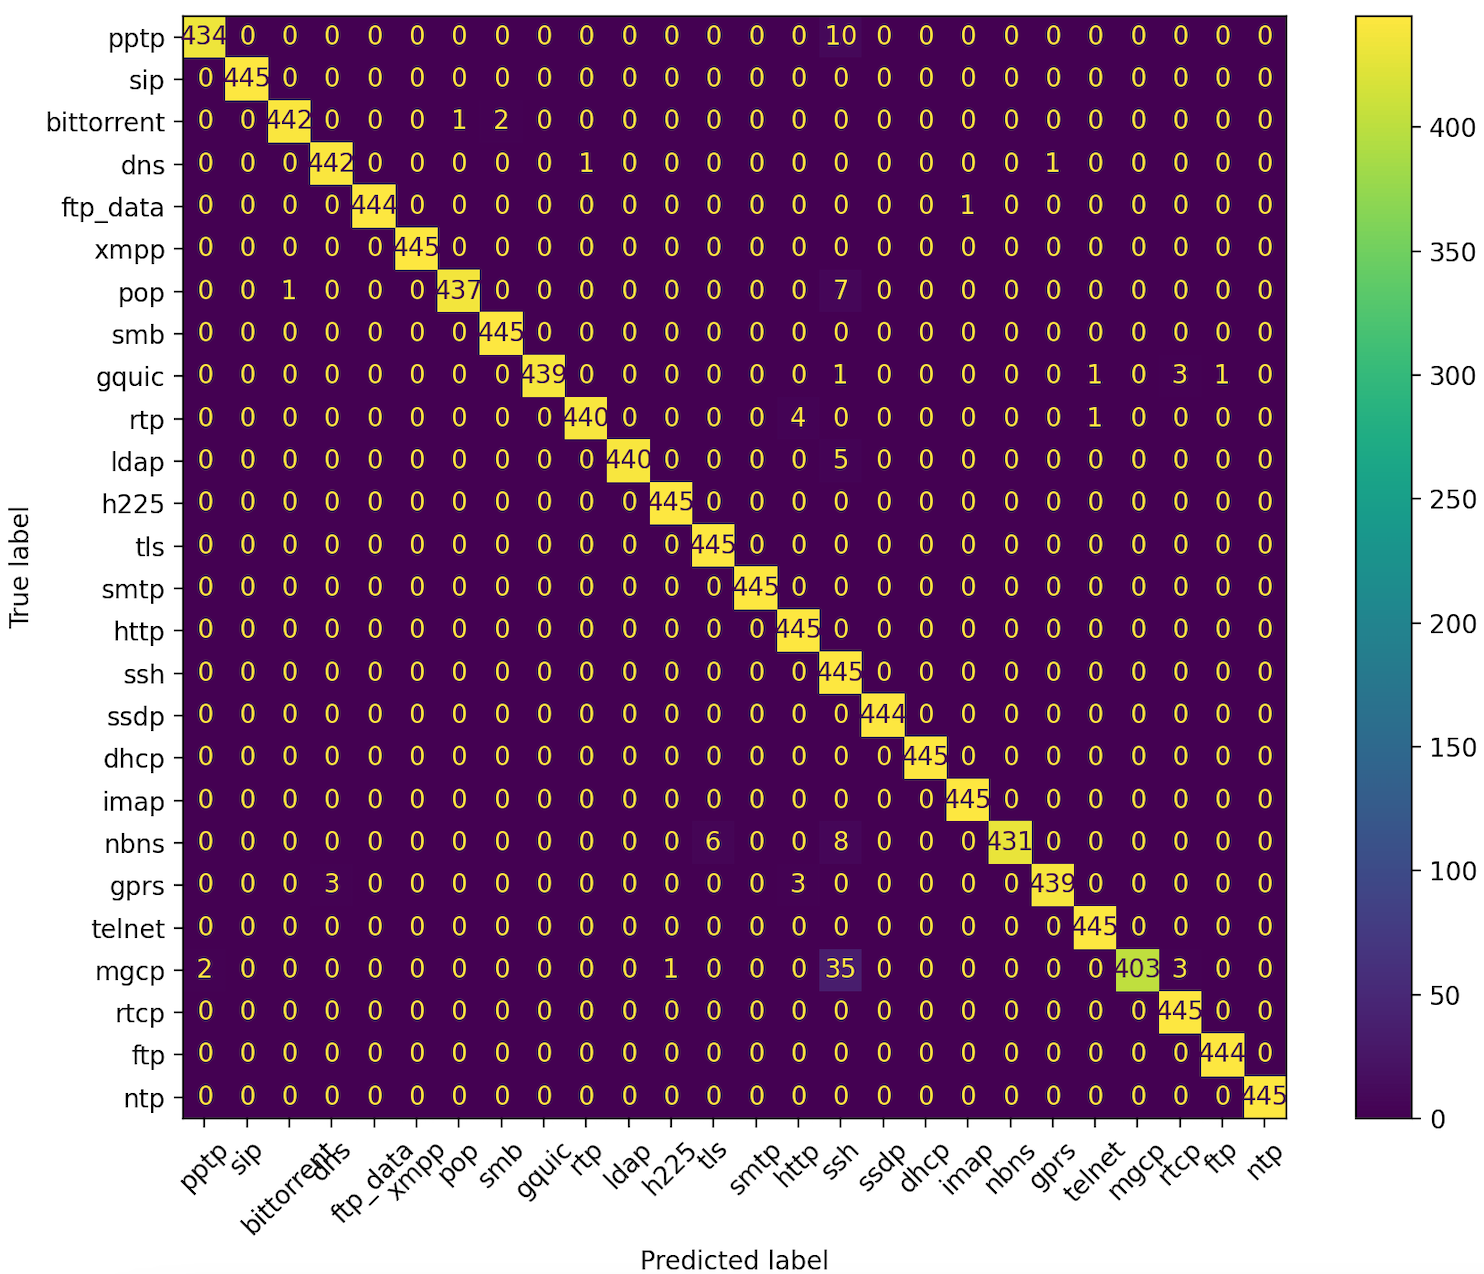
\includegraphics[width=\columnwidth]{chapters/4/img/combined.png}
  \caption{Twenty-six class identification problem using the \textsc{Alpine}-\textsc{Palm} combined model.}
  \label{fig:combined}
\end{figure}

\subsection{Traffic Type}

RFCs and standardized documentation necessitate that there are some detectable similarities between protocols. It is reasonable to think that detection of more abstract class types like traffic type (i.e. email, file transfer, web data) would be more heterogeneous and thus more difficult to embed. We experimented with classification by traffic type by amalgamating the dataset into classes as described in Table~\ref{table:dataset} in the datasets section of this work. Results in Figure~\ref{fig:trafficresults} show a confusion matrix of the classification results which are also highly accurate.

\begin{figure} [hbt!]
  \centering
  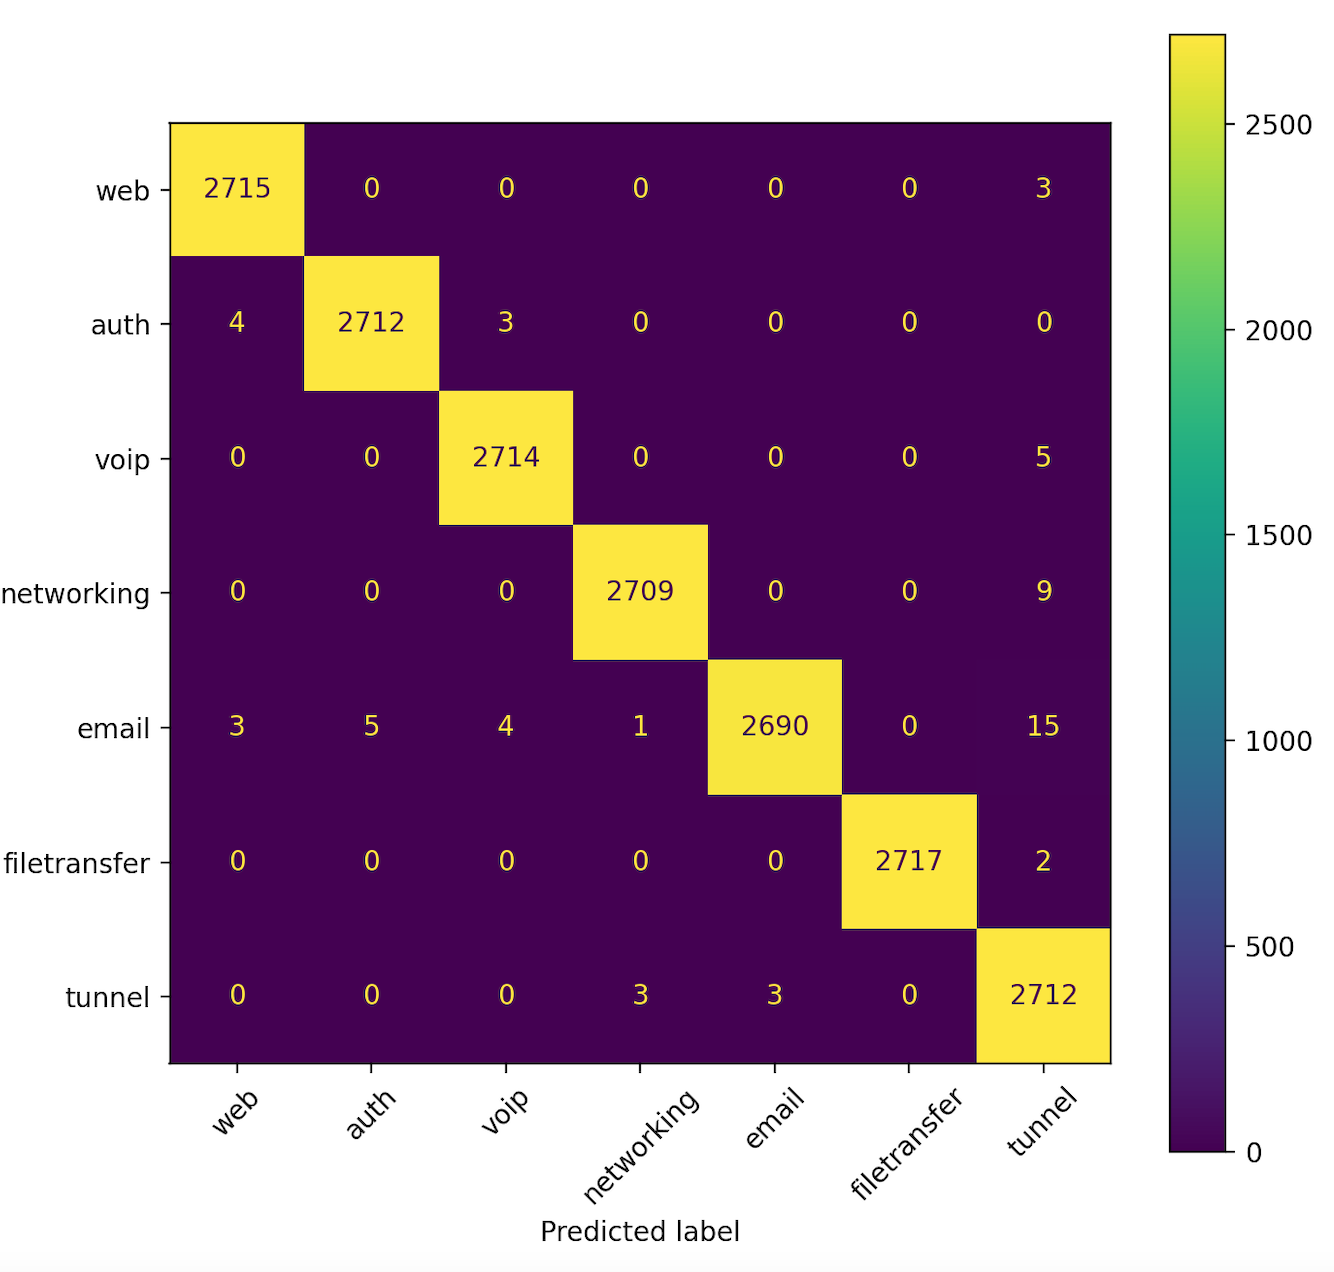
\includegraphics[width=0.8\columnwidth]{chapters/4/img/traffic_class_results.png}
  \caption{Confusion matrix of traffic type classification results.}
  \label{fig:trafficresults}
\end{figure}

\subsection{TF-IDF Score Evaluation}
In order to determine the effectivity of Jaccard similarity versus more complex similarity metrics, we evaluated the results of using payload tokens which were considered \textit{high-value} by TF-IDF score. We posed this question to address concern that large data payloads, for example HTML documents or email messages, may introduce noise into hashes which would reduce classification accuracy. Instead, isolating payload tokens to only the high value ones could reduce spurious extra data. In order to test this, we implemented a TF-IDF measurement of tokens in the training stage. This was done by modifying configurations of the PALM model to filter the added tokens. When training and test signatures were generated, only those tokens with TF-IDF score above the minimum threshold were kept and included in the actual LSH signature. The results in Table~\ref{table:results1} show that this actually had a negative impact on the overall result, indicating the basic Jaccard similarity was a better distance metric for this use case.

\subsection{LSH Multi-Embeddings}

\begin{table}
\caption{Multi-Hash Embedding Classification Results}
\centering
\begin{tabular}{| p{2cm} | p{0.6cm} p{0.6cm} p{0.6cm} || p{0.6cm} p{0.6cm} p{0.6cm} || p{0.6cm} p{0.6cm} p{0.6cm}|}
\hline
& \textbf{ALPINE} & & & \textbf{PALM} & & & \textbf{Multi-Model} & & \\
\hline
\hline
\textbf{Accuracy} & 0.988 & & & 0.717 & & & 0.996 & & \\
\textbf{Cohen's~$\kappa$} & 0.988 & & & 0.705 & & & 0.997 & & \\
\hline
\hline
 \textbf{Protocol} & \textbf{F1} & \textbf{P} & \textbf{R} & \textbf{F1} & \textbf{P} & \textbf{R} & \textbf{F1} & \textbf{P} & \textbf{R} \\
 \hline
 BitTorrent & 0.98 & 0.97 & 1.00 & 0.74 & 0.75 & 0.73 & 0.99 & 1.00 & 0.99 \\
 DHCP & 1.00 & 1.00 & 1.00 & 0.91 & 0.83 & 1.00 & 1.00 & 1.00 & 1.00 \\
 DNS & 1.00 & 1.00 & 1.00 & 0.24 & 0.46 & 0.17 & 1.00 & 1.00 & 0.99 \\
 FTP & 0.96 & 0.97 &  0.94 & 0.90 & 0.83 & 0.98 & 0.99 & 0.99 & 1.00 \\
 FTPDATA & 1.00 & 1.00 & 1.00 & 0.20 & 0.37 & 0.13 & 1.00 & 1.00 & 1.00 \\
 GPRS & 1.00 & 1.00 & 1.00 & 0.91 & 0.98 & 0.85 & 1.00 & 1.00 & 1.00 \\
 GQUIC & 0.99 & 0.99 & 1.00 & 0.27 & 0.48 & 0.19 & 0.99 & 1.00 & 0.98 \\
 HTTP & 0.99 & 1.00 & 1.00 & 0.61 & 0.65 & 0.55 & 1.00 & 1.00 & 0.99 \\
 H.225 & 1.00 & 1.00 & 1.00 & 0.63 & 0.68 & 0.95 & 1.00 & 1.00 & 0.99 \\
 IMAP & 0.99 & 0.94 & 0.98 & 0.85 & 0.77 & 0.59 & 0.99 & 1.00 & 0.99 \\
 LDAP & 0.96 & 1.00 & 0.98 & 0.66 & 0.75 & 0.59 & 0.99 & 1.00 & 0.99 \\
 MGCP & 1.00 & 1.00 & 1.00 & 0.90 & 0.83 & 1.00 & 1.00 & 1.00 & 1.00 \\
 NBNS & 0.99 & 0.98 & 1.00 & 0.87 & 0.82 & 0.92 & 0.99 & 0.99 & 1.00 \\
 NTP & 1.00 & 1.00 & 1.00 & 0.90 & 0.82 & 0.99 & 1.00 & 1.00 & 1.00 \\
 POP & 0.99 & 0.98 & 0.99 & 0.26 & 0.41 & 0.20 & 0.99 & 0.98 & 1.00 \\
 PPTP & 0.99 & 0.98 & 0.99 & 0.49 & 0.33 & 1.00 & 0.98 & 0.95 & 1.00 \\
 RTCP & 1.00 & 1.00 & 1.00 & 0.92 & 0.85 & 1.00 & 1.00 & 1.00 & 1.00 \\
 RTP & 0.99 & 0.98 & 0.99 & 0.40 & 0.65 & 0.29 & 1.00 & 1.00 & 1.00 \\
 SIP & 1.00 & 1.00 & 1.00 & 0.93 & 0.87 & 1.00 & 1.00 & 1.00 & 1.00 \\
 SMB & 0.99 & 1.00 & 0.98 & 0.81 & 0.80 & 0.82 & 0.98 & 1.00 & 0.97 \\
 SMTP & 0.98 & 0.99 & 0.98 & 0.81 & 0.80 & 0.82 & 0.99 & 1.00 & 0.99 \\
 SSDP & 0.99 & 1.00 & 0.98 & 0.92 & 0.86 & 1.00 & 1.00 & 1.00 & 1.00 \\
 SSH & 0.95 & 0.97 & 0.92 & 0.47 & 0.67 & 0.37 & 0.99 & 1.00 & 0.98 \\
 Telnet & 0.99 & 0.98 & 1.00 & 0.80 & 0.75 & 0.85 & 0.99 & 0.99 & 1.00 \\
 TLS & 0.99 & 0.99 & 1.00 & 0.61 & 0.51 & 0.75 & 1.00 & 1.00 & 1.00 \\
 XMPP & 1.00 & 1.00 & 0.99 & 0.92 & 1.00 & 0.85 & 1.00 & 1.00 & 1.00 \\
 \hline
\end{tabular}
\label{table:embeddingresults}
\end{table}

The concatenation of multiple classifiers and agreeance among voters in an ensemble has yielded a reduction in error and at best correlation when there is a misclassification~\cite{tumerensemble}. We hypothesized that enabling both \textsc{Alpine} and \textsc{Palm} to run together would yield the most accurate and agreed-upon classification results. In order to test this, we ran the 26-class protocol identification test against configurations of the model with just \textsc{Alpine} embedding, only \textsc{Palm} embedding, and a final combined run. Our results as shown in Table~\ref{table:embeddingresults} demonstrate that the combined votes of both models turned out to be the most accurate in the final tests. Furthermore, the agreeance among voters was also highest using multiple hash embeddings.

\subsection{Model Performance and Throughput}
One critical requirement for applied machine learning in network processing is that systems must keep up with signal processing at very high rates. Any passive system must not interfere with legitimate traffic and service. Furthermore, the software must be capable of performing the necessary processing on as much of the traffic as possible (ideally, all of it). While thinning and load-balancing solutions as well as diverting and copying traffic for offline analysis can help levy this concern, there is still the desire to employ classification solutions at real-time rates. Thus, we perform experiments to see how the system scales based on model sizes and number of classes. We measured the training time, system throughput in millibits per second (Mbps) as well as memory usage during the testing phase in megibytes (MiB). We ran all performance tests on the combined dataset consisting of 140,157 total packets. In order to avoid bias we implemented random under-sampling to even out the distribution of data, causing our total number of packets after sampling to be a fraction from the original set. For testing the number of classes, we created experiments with binary RTP/non-RTP classification, the traffic-type multiclass experiment with 8 classes/types, and the largest 26-class experiment where we identify all possible data layer protocols. In Table~\ref{table:performanceresults}, we detail the results of the experiments for a varied number of classes and sample sizes.

\begin{table*} [ht!]
\caption{Performance Results for Varied Number of Classes}
\centering
\begin{tabular}{| c | c | c | c | c | c | c | c |}
\hline
Classes & \# Hashes & \# Test Samples & Training Time & Test Time & Memory Usage & Throughput & Accuracy \\
\hline
\hline
\textbf{RTP/non-RTP} & 20,613 & 13,743 & 4.273s & 1.21ms & 470.8 MiB & 2.596 Mb\/s & 1.000 \\
\textit{Binary classification} & 2,400 & 1,600 & 0.738s & 0.866ms & 283.7 MiB & 3.139 Mb\/s & 0.997 \\
& 240 & 160 & 0.075s & 1.093ms & 353.4 MiB & 2.317 Mb\/s & 1.00 \\
\hline
\textbf{Traffic Type} & 28,543 & 19,029 & 7.136s & 1.015ms & 584.6 MiB & 3.728 Mb\/s & 0.997 \\
\textit{8-class problem} & 12,600 & 8,400 & 3.31s & 1.006ms & 305.3 MiB & 2.842 Mb\/s & 0.997 \\
& 240 & 160 & 0.683s & 2.397ms & 290.6 MiB & 2.54 Mb\/s & 0.998 \\
\hline
\textbf{Protocol} & 17,347 & 11,565 & 5.312s & 1.138ms & 352.4 MiB & 3.041 Mb\/s & 0.997 \\
\textit{26-class problem} & 15,600 & 10,400 & 3.13s & 0.727ms & 305.3 MiB & 4.231 Mb\/s & 0.998 \\
& 1,560 & 1,040 & 0.492s & 0.901ms & 301.8 MiB & 3.212 Mb\/s & 0.994 \\
\hline
\end{tabular}
\label{table:performanceresults}
\end{table*}

In order to test system scalability in deployment and verify the theoretical complexity discussed in the background section of this work, we performed a series of experiments increasing the number of signatures for a model used to classify HTTP traffic. As a comparator, we used the regular expression scanning tool built in RExACtor which uses the Hyperscan 5.4.0 regular expression matching library by Intel~\cite{hyperscan}. All experiments were performed on a single i9 Dell computer with Ubuntu 18.04 installed. In the trials, the number of signatures represented the number of LSH hashes our system or the number of regular expressions added to the sniffer application. We used RExACtor~\cite{rexactor} to generate HTTP signatures from the HTTP traffic in our dataset. Both models performed the classification with 100\% accuracy on all trials.

\begin{table}[ht!]
\centering
\begin{tabular}{| c | c | c | c | c |}
\hline
System & \# Signatures & Training & Testing & Memory \\
\hline
\hline
\textbf{ALPINE/PALM} & 1,000 &  1.21s &  1.23s & 392.4 MiB \\
& 10,000 & 2.75s & 3.56s & 419.9 MiB \\
& 100,000 & 52.75s & 4.2s & 1047.4 MiB \\
& 1,000,000 & 423.3s & 4.52s & 4717.9 MiB \\
\hline
\textbf{Hyperscan} & 1,000 & 4.6s & 156ms & 70.7 MiB \\
& 10,000 & 81.8s & 1.3s & 529.3 MiB \\
& 100,000 & 39.9m & 17.28s & 4596.7 MiB \\
& 1,000,000 & 153m & 63.1s & - \\
\hline
\end{tabular}
\caption{Performance Results for \textsc{Alpine} and \textsc{Palm} as a multi-embedding versus Hyperscan}
\label{table:performanceresults}
\end{table}

\begin{figure} [ht!]
  \centering
  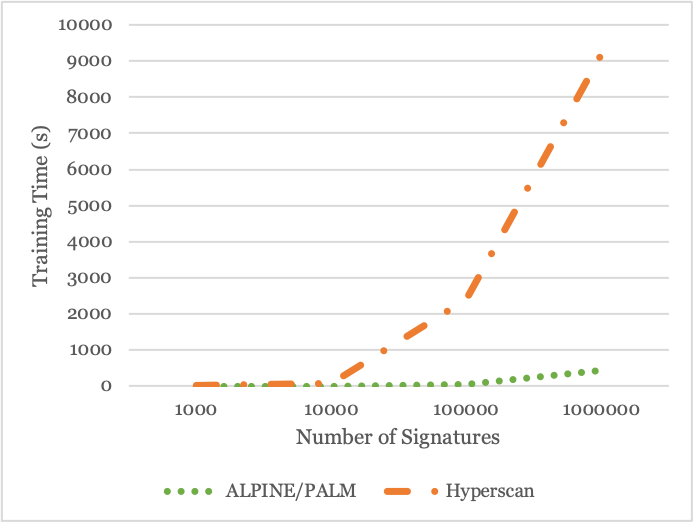
\includegraphics[width=0.6\columnwidth]{chapters/4/img/trainingtime.png}
  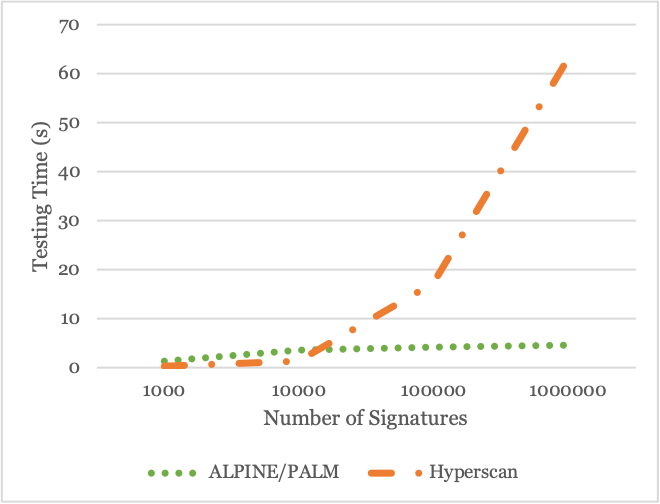
\includegraphics[width=0.6\columnwidth]{chapters/4/img/testingtime.png}
  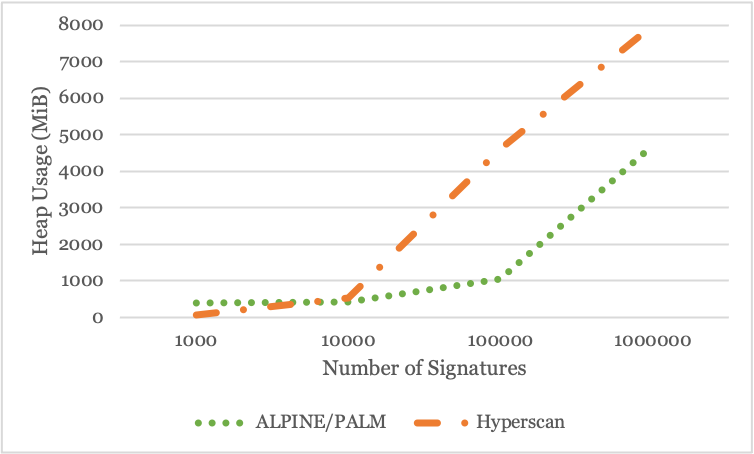
\includegraphics[width=0.6\columnwidth]{chapters/4/img/memoryusage.png}
  \caption{Time and space complexity results for \textsc{Alpine}/\textsc{Palm} versus Hyperscan.}
  \label{fig:hyperscancompare}
\end{figure}
